\subsection{Nonlinear shoaling wave over submerged bar}
In this laboratory experiment an incident sin wave travels over a trapezoidal underwater obstacle and the surface elevations of the non-breaking wave are measured at several gauges spread along the obstacle.
This experiment conducted in different versions by \cite{BejiBattjes.1993} and \cite{BejiBattjes.1994}, \cite{Dingemans.1994} (more cases, here only case A considered), and by Luth et al. (1994) (cited in \cite{Dingemans.1994}, but I do not have access to the report). 
In this experiments, gauges and setups were different (see tables \ref{tab:bejibattjes_gauges_SZ} -- \ref{tab:bejibattjes_gauges_BB1994} and figures \ref{fig:bejibattjes_setup_SZ} -- \ref{fig:bejibattjes_setup_BB1994}).

The setup is as described in \cite{StellingZijlema.2003}, and M. Zijlema provided the data. According to the gauges, this should be the data described in \cite{Dingemans.1994, StellingZijlema.2003} as the data from Luth et al. (1994), but scaled (divided) by a factor of 2. 

The initial condition is the unperturbed state. The boundary condition is described as in incident wave at the left boundary of the computational domain, where the surface elevation is set to $\xi=a \text{sin}\left(\frac{2\pi t}{T}\right)$ with period $T=2.02 \,$s and amplitude $a=1.0\,$cm.
We impose reflecting boundary conditions at the boundary in x-direction and periodic boundary conditions in y-direction. For the setup see figure \ref{fig:bejibattjes_setup_SZ}. The computational domain is enlarged to 40m to ensure no reflecting waves disturbing the solution during the simulation time of 40s.

Note: No boundary conditions are specified for w and q at the moment, computations which set them to zero are running. This hopefully explains the wrong behavior. 


\begin{table}[htbp]
\begin{tabular}{lllllllll}
\textbf{gauge} & G4 & G5 & G6 & G7 & G8 & G9 & G10 & G11 \\
\toprule
\textbf{x [m]} & 10.5 & 12.5 & 13.5 & 14.5 & 15.7 & 17.3 & 19.9 & 21.0 \\
\bottomrule
\end{tabular}
\caption{Locations of gauges used in \cite{StellingZijlema.2003}}
\label{tab:bejibattjes_gauges_SZ}
\end{table}

\begin{table}[htbp]
\begin{tabular}{lllllllll}
\textbf{gauge} & 1 & 2 & 3 & 4 & 5 & 6 & 7 & 8 \\
\toprule
\textbf{x [m]} & 6.0 & 11.0 & 12.0 & 13.0 & 14.0 & 15.0 & 16.0 & 17.0 \\
\bottomrule
\end{tabular}
\caption{Locations of gauges used in \cite{BejiBattjes.1993}}
\label{tab:bejibattjes_gauges_BB1993}
\end{table}

\begin{table}[htbp]
\begin{tabular}{llllllll}
\textbf{gauge} & 1 & 2 & 3 & 4 & 5 & 6 & 7 \\
\toprule
\textbf{x [m]} & 6 & 10.8 & 12.8 & 13.8 & 14.8 & 16.0 & 17.6 \\
\bottomrule
\end{tabular}
\caption{Locations of gauges used in \cite{BejiBattjes.1994}}
\label{tab:bejibattjes_gauges_BB1994}
\end{table}

\begin{figure}[htbp]
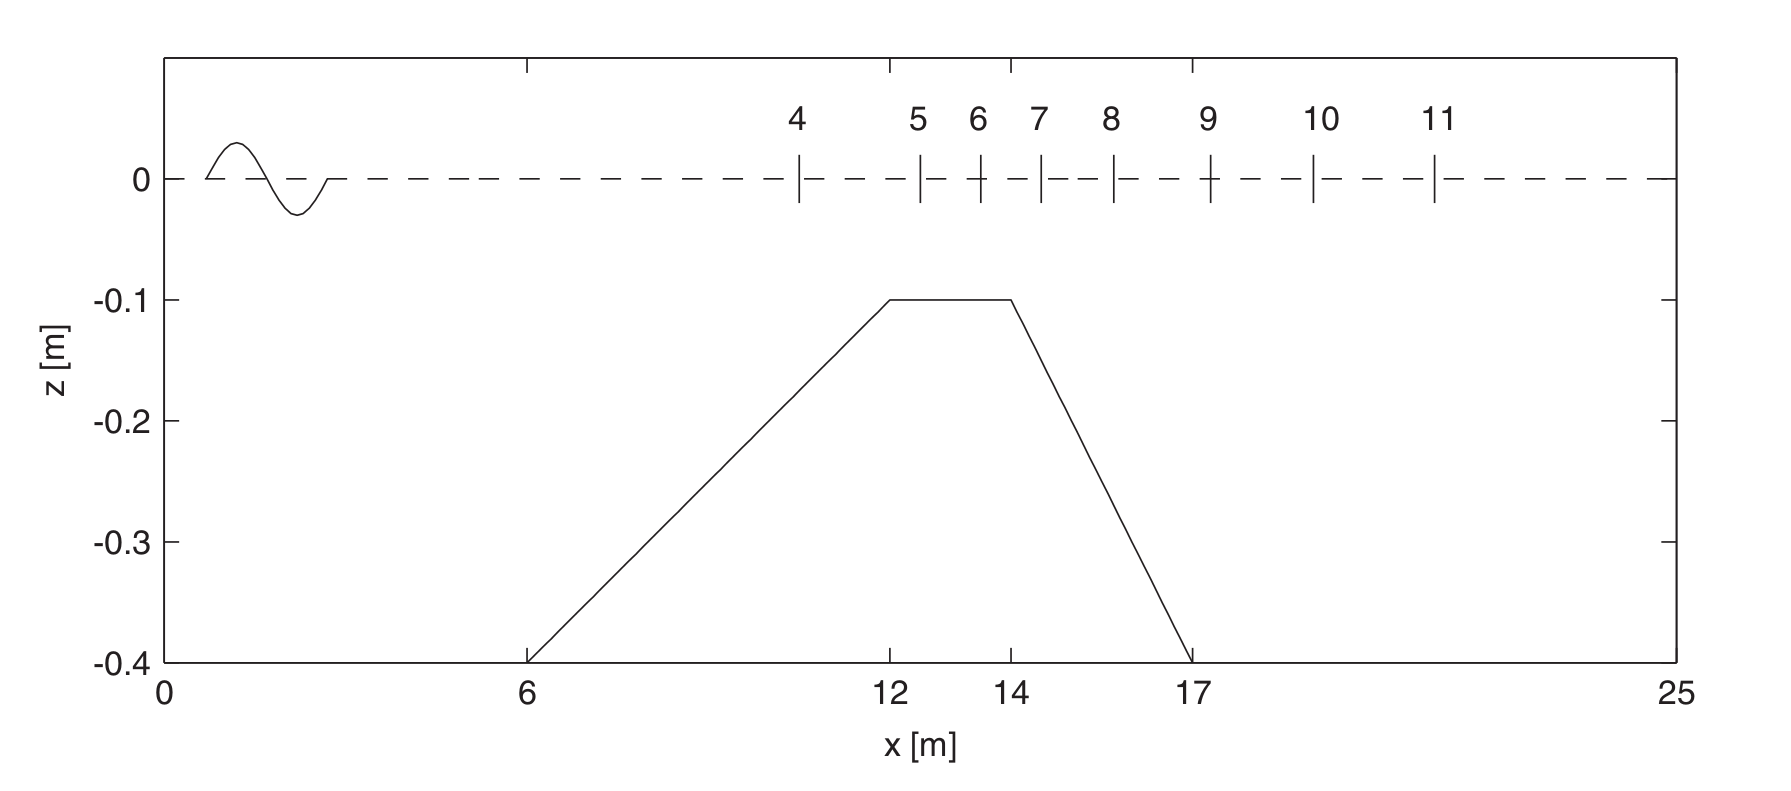
\includegraphics[width=\textwidth]{bejibattjes_setup_SZ}
\caption{Setup of the experiment of Beji and Battjes according to \cite{StellingZijlema.2003}}
\label{fig:bejibattjes_setup_SZ}
\end{figure}

\begin{figure}[htbp]
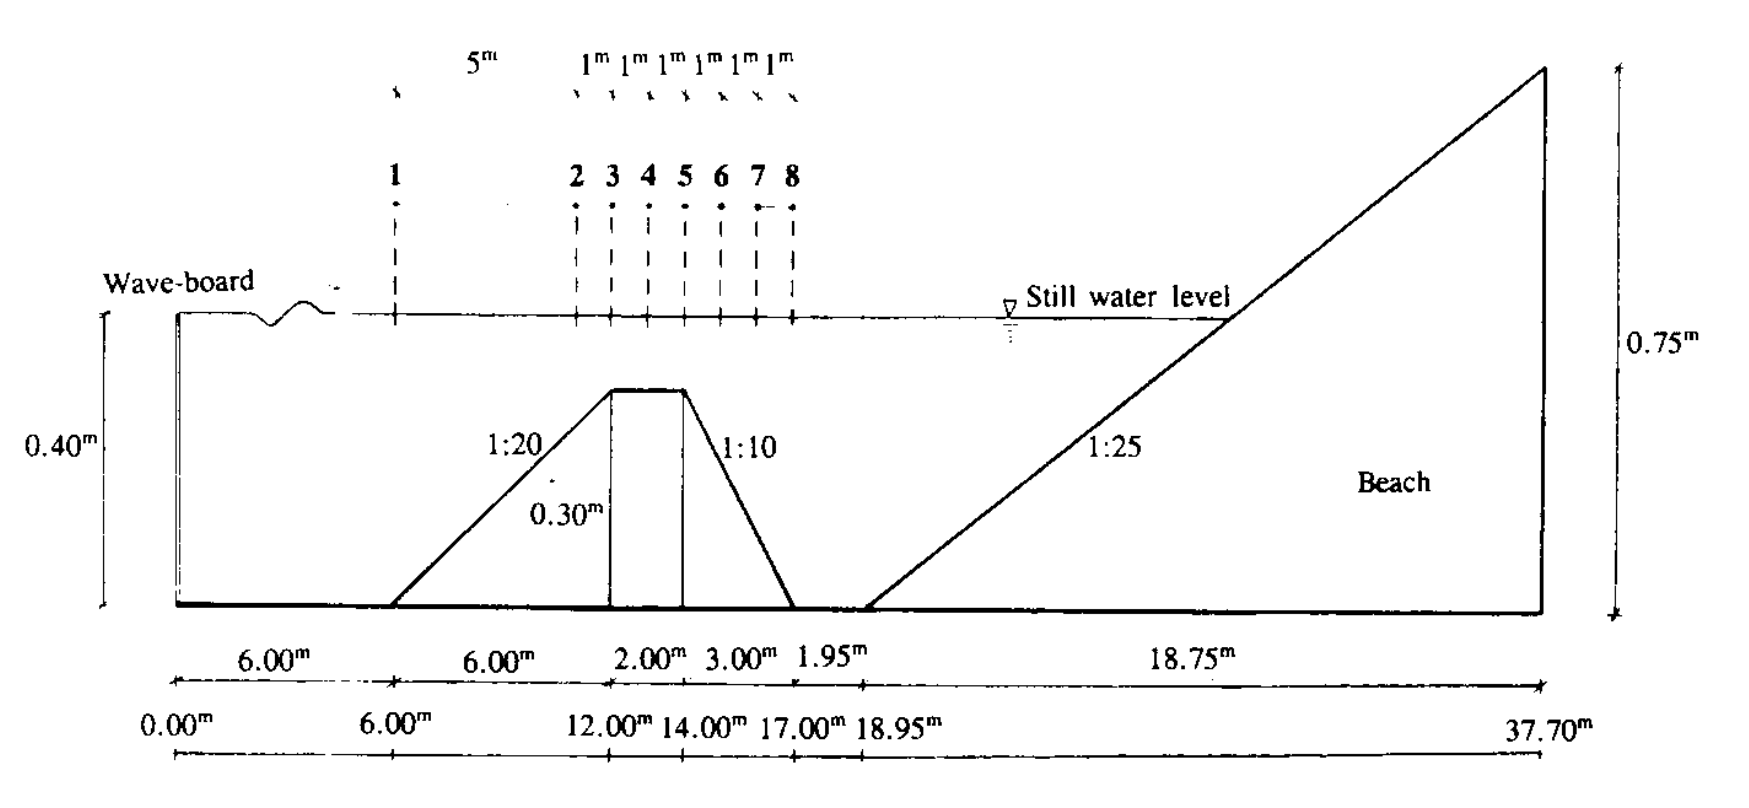
\includegraphics[width=\textwidth]{bejibattjes_setup_BB1993}
\caption{Setup of the experiment of Beji and Battjes according to \cite{BejiBattjes.1993}}
\label{fig:bejibattjes_setup_BB1993}
\end{figure}

\begin{figure}[htbp]
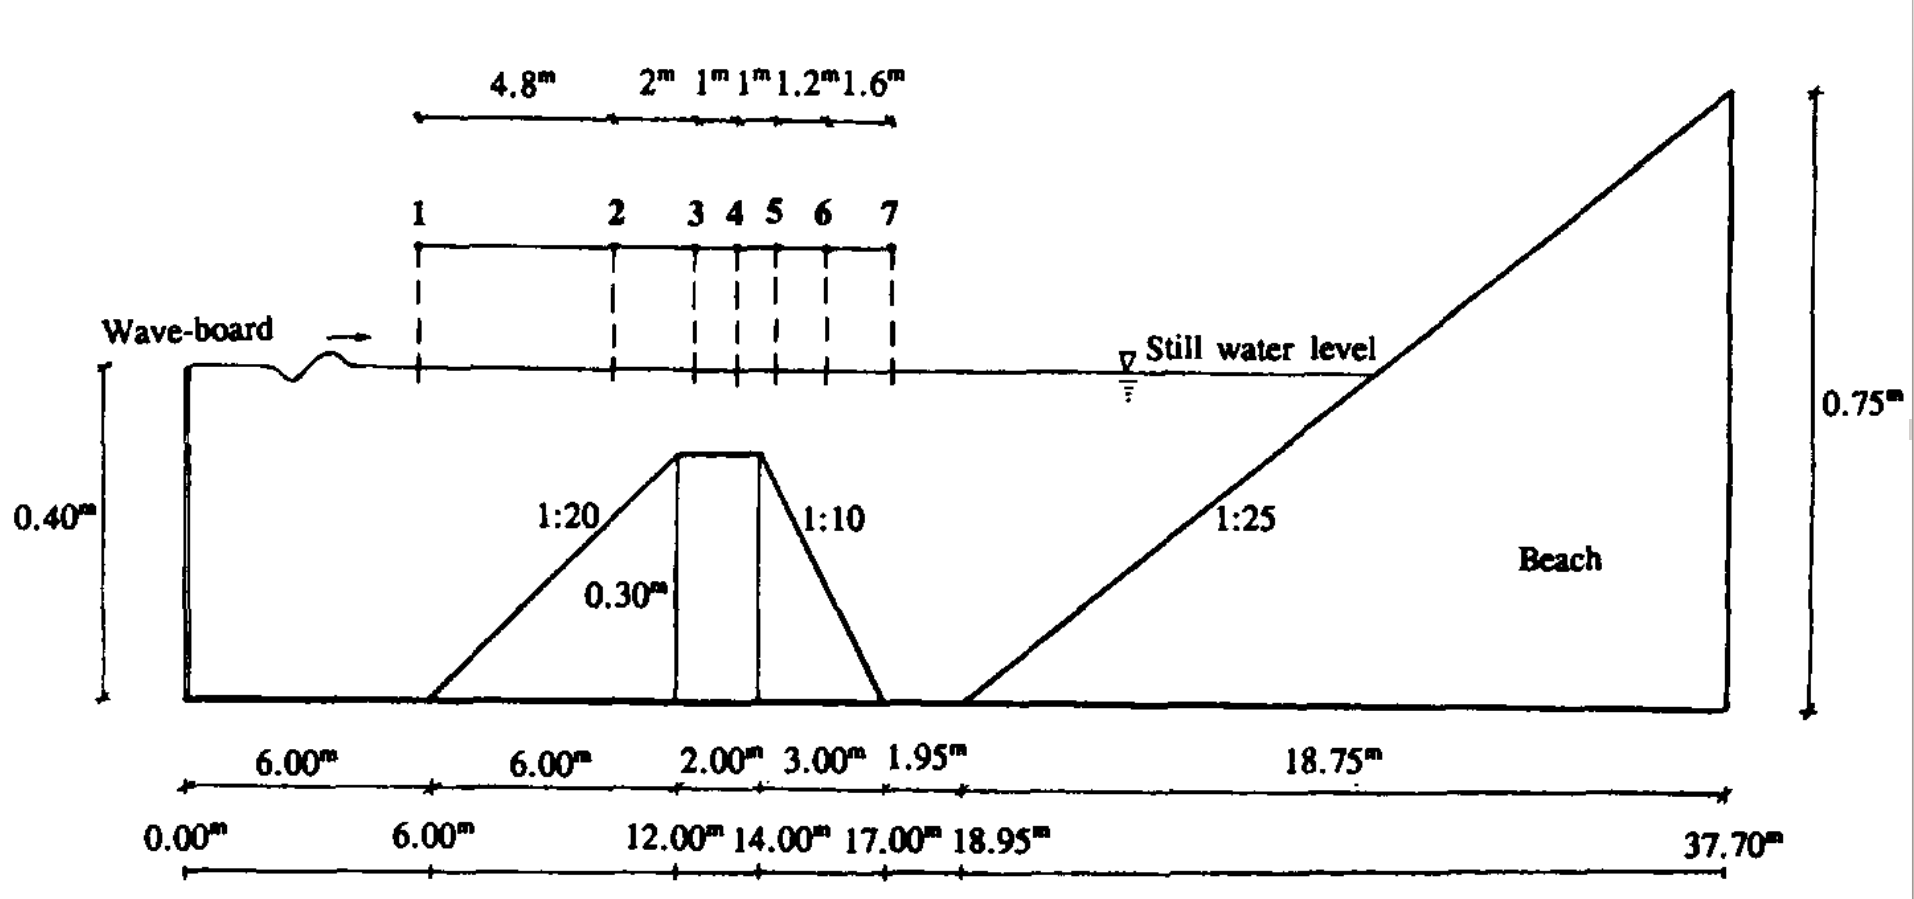
\includegraphics[width=\textwidth]{bejibattjes_setup_BB1994}
\caption{Setup of the experiment of Beji and Battjes according to \cite{BejiBattjes.1994}}
\label{fig:bejibattjes_setup_BB1994}
\end{figure}

\subsubsection{Results of \nh\ model}
The model results can be found in figure \eqref{fig:nh_bejjibattjes_nh}.
The results are shifted in time by 4.5s to match the laboratory data at gauge 10 in phase after 20s.

\begin{figure}[htbp]
\begin{minipage}{\textwidth}
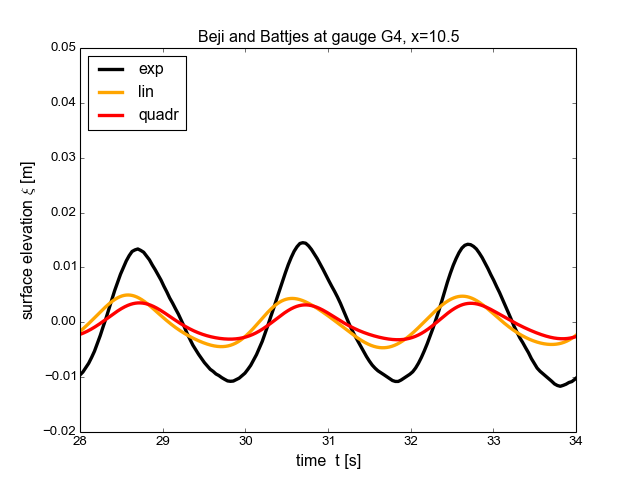
\includegraphics[width=0.48\textwidth]{BejiBattjes_nh_x=loc_4}
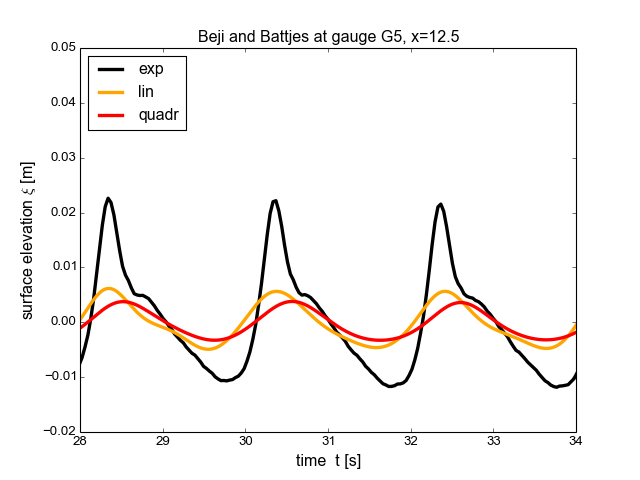
\includegraphics[width=0.48\textwidth]{BejiBattjes_nh_x=loc_5}
\end{minipage} \\
\begin{minipage}{\textwidth}
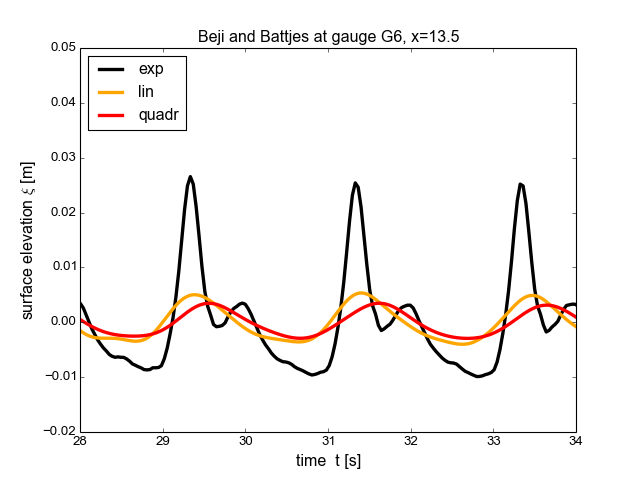
\includegraphics[width=0.48\textwidth]{BejiBattjes_nh_x=loc_6}
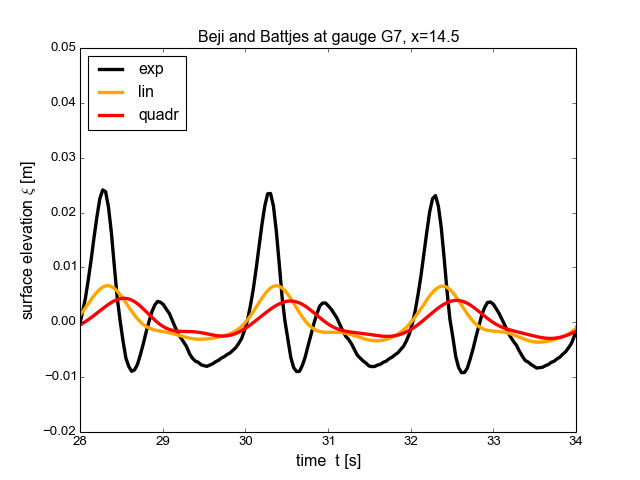
\includegraphics[width=0.48\textwidth]{BejiBattjes_nh_x=loc_7}
\end{minipage} \\
\begin{minipage}{\textwidth}
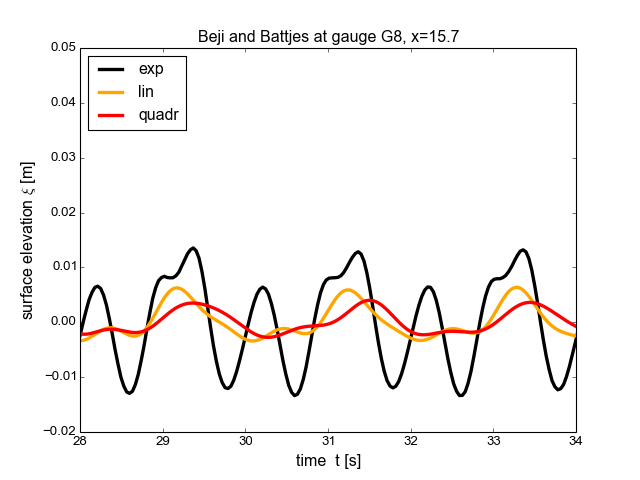
\includegraphics[width=0.48\textwidth]{BejiBattjes_nh_x=loc_8}
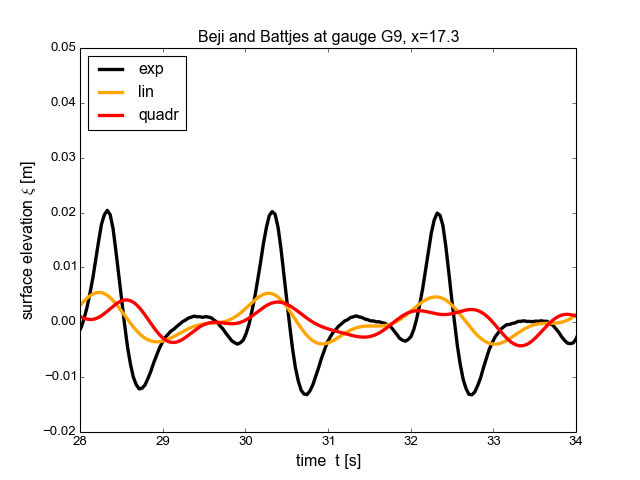
\includegraphics[width=0.48\textwidth]{BejiBattjes_nh_x=loc_9}
\end{minipage} \\
\begin{minipage}{\textwidth}
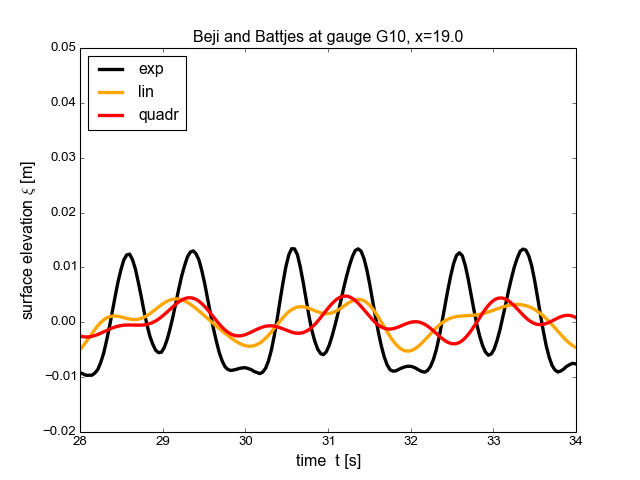
\includegraphics[width=0.48\textwidth]{BejiBattjes_nh_x=loc_10}
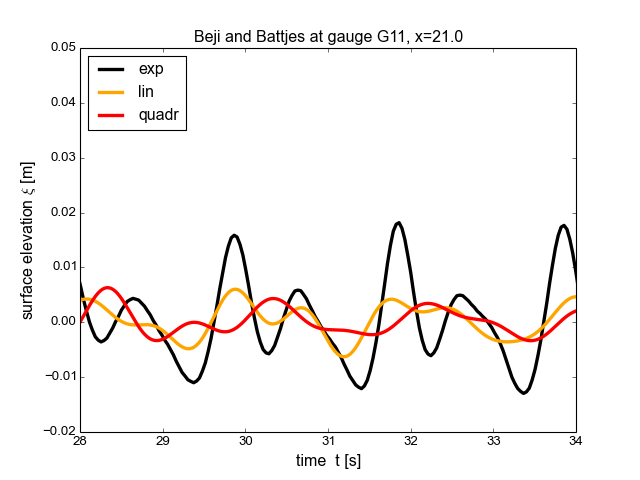
\includegraphics[width=0.48\textwidth]{BejiBattjes_nh_x=loc_11}
\end{minipage}
\caption{Comparison of the laboratory (black) sea surface height at gauges with the simulation results of the \nh\ model with linear pressure profile (yellow) and quadratic pressure profile (red)}
\label{fig:nh_bejjibattjes_nh}
\end{figure}